% Ported verbatim (prose unchanged) from docs/SECTION_4_DRAFT.md.
% MELD dataset citation (Poria et al., 2019) resolved: docs/CITATIONS.md's
% update added the real entry (poria2019meld).
\section{MELD Experiments}
\label{sec:meld}

This section establishes the paper's central empirical claim on MELD: conversation-graph machinery yields real, replicable gains when the utterance encoder is frozen, and those gains vanish (indeed, reverse in sign) once the encoder is fine-tuned, even when the fine-tuned encoder sees no conversational context at all. The argument proceeds in the order the evidence demands: the experimental setup and the feature landscape any architecture must work within (\ref{sec:meld-setup}), the frozen-feature regime in which the literature's premise is reproduced (\ref{sec:meld-frozen}), the fine-tuned regime in which it fails (\ref{sec:meld-finetuned}), the context-window sweep separating the effect of fine-tuning from the effect of contextual input (\ref{sec:k-sweep}), and the mechanism analysis explaining why scratch-retrained ablations overstate the harm that residual attribution measures precisely (\ref{sec:meld-mechanism}).

\subsection{Setup and the Feature Landscape}
\label{sec:meld-setup}

MELD~\cite{poria2019meld} comprises roughly $13{,}000$ utterances from $1{,}432$ multi-party dialogues drawn from the television series \textit{Friends}, each labeled with one of seven emotions under severe class imbalance: the majority class (neutral) accounts for $48.1\%$ of the test set, while the two rarest classes, fear and disgust, have $50$ and $68$ test instances respectively. We use the standard splits. All models are evaluated by weighted F1 (primary, for literature comparability) and macro F1, with per-class scores reported for the rare classes throughout; a constant all-neutral classifier scores $0.313$ weighted F1 and anchors the bottom of every comparison.

Before any architecture is trained, we characterize the features it will consume with linear probes: a logistic-regression classifier per modality, utterance-level, no conversational context. On frozen features (masked-mean RoBERTa-base embeddings for text, mean-pooled Wav2Vec~2.0 for audio, mean-pooled MViTv2 over eight frames for video), the probes reach $0.527$, $0.411$, and $0.335$ weighted F1 respectively, with the three-modality concatenation at $0.525$, marginally \textit{below} text alone (Table~\ref{tab:meld-probe}). Two observations from this table shape everything downstream. First, text dominates: on MELD, the non-textual modalities offer any architecture at most a few points of headroom, and naive feature concatenation already fails to realize it. Second, the modalities are not redundant for the rare classes: under class-balanced probing (a classifier trained with \texttt{class\_weight=`balanced'}, evaluated with the same weighted F1 as above; ``balanced'' describes the training setting, not a different metric) the concatenation ($0.460$) clearly exceeds text alone ($0.428$), indicating that acoustic and visual signal exists disproportionately where text is weakest. The question the rest of this section asks is whether graph-structured context modeling can convert any of this into utterance-level performance, and against which foundation.

\begin{table}[t]
\centering
\caption{MELD frozen-feature linear probes (weighted F1). ``Balanced'' trains with \texttt{class\_weight=`balanced'}; both columns report weighted F1 (not a different metric).}
\label{tab:meld-probe}
\begin{tabular}{lcc}
\toprule
row & unbalanced & balanced \\
\midrule
all-neutral (constant) & 0.3127 & 0.3127 \\
random-stratified & 0.2914 & 0.2914 \\
video & 0.3349 & 0.1931 \\
audio & 0.4111 & 0.2971 \\
text & 0.5274 & 0.4277 \\
concat & 0.5250 & 0.4604 \\
\bottomrule
\end{tabular}
\par\footnotesize Metric: weighted\_f1.
\end{table}


\subsection{The Frozen Regime: The Literature's Premise, Reproduced}
\label{sec:meld-frozen}

The graph-ERC literature's implicit experimental contract is a frozen or lightly adapted encoder beneath a trained contextual architecture. We instantiate that contract under our attribution methodology: a frozen-feature textual foundation (a linear classifier over the frozen text embeddings, trained with the locked recipe; test weighted F1 $0.4416$ under macro-F1 selection) provides the residual anchor, and the full graph stack (multimodal fusion, speaker-state recurrence, relational memory, shift objective, temporal attention) is trained on top under the zero-initialized residual construction of Section~\ref{sec:residual-construction}, three seeds, with equality-at-init verified against the frozen foundation before launch.

The result reproduces the literature's premise cleanly: the graph stack's paired per-seed gain over its own foundation is $\mathbf{+0.0356 \pm 0.0106}$, positive, larger than three standard deviations, consistent in sign across all seeds (Table~\ref{tab:frozen-bridging}). On frozen features, conversation-graph machinery works. This is not a strawman reproduction: the gain is measured under the most conservative attribution instrument we have, one that (Section~\ref{sec:meld-finetuned}) reports \textit{nulls} where scratch retraining reports harms, so the $+0.036$ cannot be attributed to optimization disturbance. We note one caveat for completeness: the frozen anchor's absolute level ($0.4416$) is depressed relative to the sklearn probe on the same features ($0.5274$) by the macro-F1 selection rule applied uniformly across this study; the paired comparison is internally consistent because anchor and stack share the selection rule, and the fine-tuned regime below uses the identical rule and nevertheless produces nulls.

\begin{table*}[t]
\centering
\caption{Frozen-regime bridging experiment: paired per-seed gain, full\_R\_frozen minus the frozen text anchor, under the identical residual apparatus as the fine-tuned end.}
\label{tab:frozen-bridging}
\begin{tabular}{lccc}
\toprule
config & test weighted F1 & paired gain vs.\ anchor & n seeds \\
\midrule
frozen text anchor (seed 42) & 0.4416 & -- & 1 \\
base\_fusion\_R\_frozen & 0.5290 $\pm$ 0.0013 & -- & 3 \\
full\_R\_frozen & 0.4773 $\pm$ 0.0106 & +0.0356 $\pm$ 0.0106 & 3 \\
\bottomrule
\end{tabular}
\end{table*}


\subsection{The Fine-Tuned Regime: The Premise Fails}
\label{sec:meld-finetuned}

We then replace only the foundation. The LoRA-fine-tuned contextual text encoder of Section~\ref{sec:meld-foundation} (test weighted F1 $0.6403 \pm 0.0045$, itself exceeding the published full-system performance of DialogueRNN, MMGCN, EmoShiftNet~\cite{dialoguernn2019,mmgcn2021,emoshiftnet2025}, and our own prior SocialArcNet (published: $0.62$ weighted F1)~\cite{socialarcnet2026}, on this benchmark) supplies the anchor logits and embeddings; the architectural stack, the acoustic and visual features, the residual construction, the recipe, and the seeds are unchanged. Two experimental designs bracket the question.

Under conventional scratch retraining (every configuration trained from random initialization, the design of standard ablation studies), the ordering \textit{inverts}: the plain fusion baseline is the best configuration in the matrix, and the full graph stack lands $0.0129$ below it and $0.0175$ below the text-only anchor, with the deficit consistent across weighted F1, macro F1, and the rare-class scores the components specifically target. Under residual attribution, the picture is cleaner and more precise: the full stack's paired gain over its own fusion baseline is $\mathbf{-0.0048}$ at the locked context width, and over the fine-tuned text anchor $\mathbf{-0.0060}$, and the seven-seed endpoint analysis of Section~\ref{sec:k-sweep} places it at $-0.0088 \pm 0.0072$, a null-to-slightly-negative contribution, incompatible with the $+0.0356$ measured on frozen features by the identical instrument. The component-resolved ablations attribute the residue consistently: removing the relational memory from the full stack \textit{improves} every aggregate metric we checked (weighted F1 by $0.0022$, macro F1 by $0.0023$, and both rare classes: fear by $0.0024$, disgust by $0.0084$, means of $3$ seeds), and no single component's isolated contribution is positive beyond seed noise.

\begin{table}[t]
\centering
\caption{MELD, fine-tuned foundation: scratch retraining (N4) vs.\ residual attribution (N4-R). The full-stack deficit shrinks 63\% under residual attribution.}
\label{tab:scratch-vs-residual}
\begin{tabular}{lcc}
\toprule
 & scratch (N4) & residual (N4-R) \\
\midrule
baseline (fusion only) & 0.6356 $\pm$ 0.0013 & 0.6392 $\pm$ 0.0011 \\
full stack & 0.6228 $\pm$ 0.0155 & 0.6344 $\pm$ 0.0061 \\
gap (full $-$ baseline) & -0.0129 & -0.0048 \\
\bottomrule
\end{tabular}
\end{table}

\begin{table*}[t]
\centering
\caption{Per-class test F1 (mean of 3 seeds), MELD. Rare classes in \textbf{bold}.}
\label{tab:per-class-meld}
\begin{tabular}{lcccc}
\toprule
class & Text-only anchor & Fusion & Full stack (no relational) & Full stack \\
\midrule
neutral & 0.799 & 0.800 & 0.797 & 0.793 \\
joy & 0.613 & 0.613 & 0.610 & 0.607 \\
sadness & 0.380 & 0.357 & 0.367 & 0.369 \\
anger & 0.475 & 0.485 & 0.476 & 0.480 \\
surprise & 0.570 & 0.562 & 0.563 & 0.558 \\
\textbf{fear} & 0.129 & 0.074 & 0.082 & 0.079 \\
\textbf{disgust} & 0.166 & 0.198 & 0.188 & 0.179 \\
\bottomrule
\end{tabular}
\end{table*}


The contrast between Sections~\ref{sec:meld-frozen} and~\ref{sec:meld-finetuned} is the boundary claim, measured under uniform methodology: the same components, the same attribution instrument, the same recipe, the same seeds. The result is a $+0.036$ contribution on frozen features and a null-to-negative contribution on fine-tuned ones. What changed is the foundation, and on the evidence of Section~\ref{sec:k-sweep}, what matters about the foundation is the fine-tuning itself rather than its contextual input window.

\begin{figure}[t]
\centering
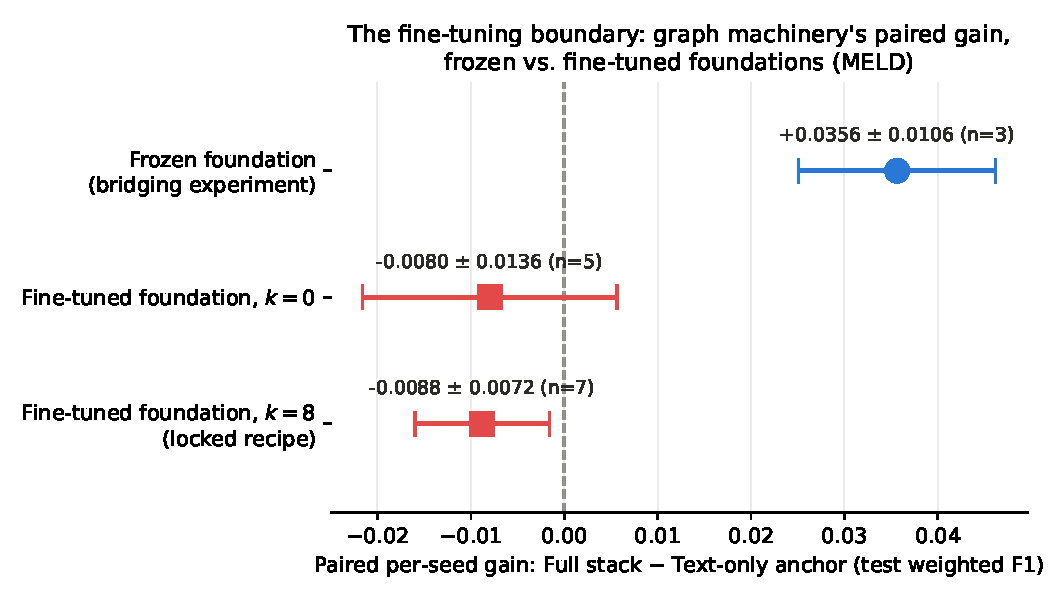
\includegraphics[width=\columnwidth]{figures/boundary_figure.pdf}
\caption{Paired per-seed gain of the Full stack over its own Text-only anchor, MELD, at three points: frozen foundation ($+0.0356$), fine-tuned foundation at context width $k=0$ ($-0.0080$), and fine-tuned foundation at $k=8$, the locked recipe ($-0.0088$). Marker shape (circle vs.\ square) distinguishes the frozen point from the two fine-tuned points independently of color; error bars are one standard deviation across seeds. The gain is positive only on the frozen foundation --- both fine-tuned endpoints are null-to-negative.}
\label{fig:boundary}
\end{figure}

\subsection{Separating Fine-Tuning from Context: The $k$-Sweep}
\label{sec:k-sweep}

A natural reading of Section~\ref{sec:meld-finetuned} would be that the contextual input window ($k=8$ preceding utterances) simply pre-empts the graph: the encoder already sees the recent dialogue, so graph-propagated context is redundant. The $k$-sweep tests this reading and finds it insufficient. We retrain the fine-tuned foundation at context widths $k \in \{0, 2, 4, 8\}$ (where $k=0$ is a genuinely context-free but still fine-tuned encoder) and measure the graph stack's paired residual gain at each width, with the endpoints powered to seven seeds (five for the $k=0$ anchor: the $k=0$ text anchor was seed-$42$-only in the original design, and this consolidation pass added the four new seeds it was asked to add, not six) and the interior points reported at one seed as trend indicators only.

At $k=8$ the gain is $-0.0088 \pm 0.0072$ (negative, exceeding one standard deviation); at $k=0$ it is $-0.0080 \pm 0.0136$ (indistinguishable from zero). Figure~\ref{fig:k-sweep} displays the curve with the endpoint error bars emphasized. The decisive cell is $k=0$: a fine-tuned encoder that has never seen a single context utterance already leaves nothing for the graph stack to add, while the \textit{frozen} encoder of Section~\ref{sec:meld-frozen}, equally context-free, left $+0.036$ on the table. Context windows are therefore not the operative variable; task-adaptation of the representation is. Whatever conversational information the graph machinery propagates on frozen features, a fine-tuned encoder either encodes it, obviates the need for it, or renders it inaccessible to the stack, and the mechanism analysis below favors a specific interpretation.

\begin{table}[t]
\centering
\caption{Context-window ($k$) sweep, MELD: paired per-seed gain (Full stack $-$ Text-only anchor) at the powered endpoints.}
\label{tab:k-sweep-endpoints}
\begin{tabular}{lccc}
\toprule
endpoint & $n$ pairs & paired gain & $|$gain$|>$std \\
\midrule
$k=0$ & 7 & -0.0072 $\pm$ 0.0128 & False \\
$k=8$ & 7 & -0.0088 $\pm$ 0.0072 & True \\
\bottomrule
\end{tabular}
\end{table}


\begin{figure}[t]
\centering
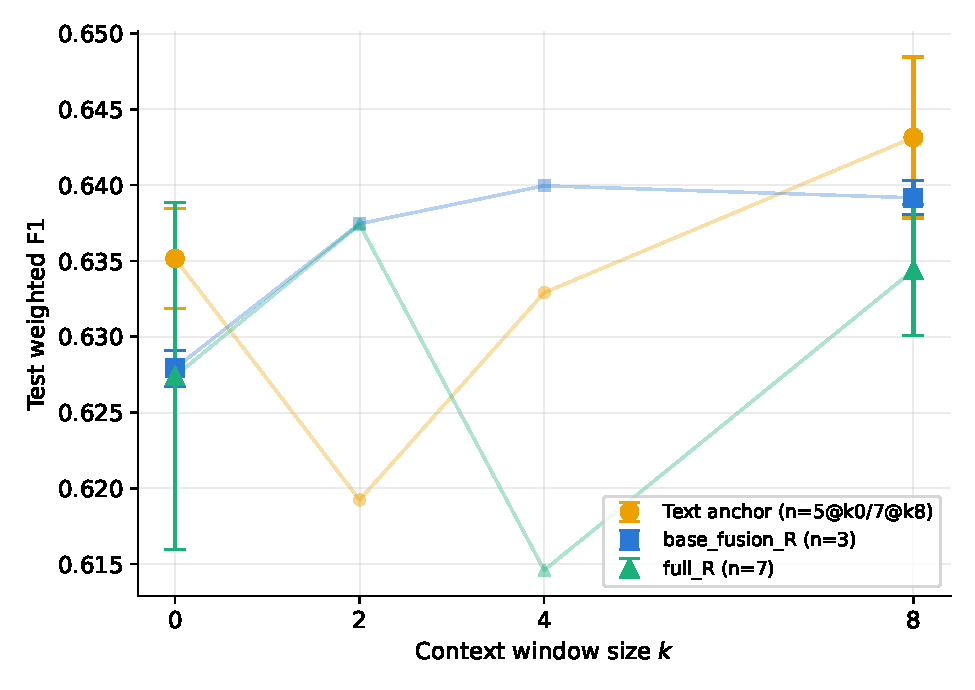
\includegraphics[width=\columnwidth]{figures/k_sweep_curve.pdf}
\caption{MELD context-window sweep: paired per-seed gain of the Full stack over its own Text-only anchor (y-axis, ``Paired gain in weighted F1'') at each context window size $k$ (x-axis, ``Context window size $k$''), $k \in \{0,2,4,8\}$. Endpoints ($k=0$, $k=8$; square markers with error bars) are multi-seed, $n=5$ and $n=7$ respectively, error bars one standard deviation; interior points ($k=2$, $k=4$; light circle markers, no error bars) are single-seed trend indicators only, de-emphasized rather than treated as estimates.}
\label{fig:k-sweep}
\end{figure}

\subsection{Mechanism: Why Scratch Ablations Overstate, and What the Stack Actually Learns}
\label{sec:meld-mechanism}

Three analyses localize the mechanism. First, overfitting: under scratch retraining the train--validation gap grows monotonically with component count ($+0.129$ for fusion alone to $+0.225$ for the full stack), and the full stack never exceeds the fusion baseline's peak validation performance at any epoch in any seed: the components' scratch-measured harm is substantially an optimization-and-capacity artifact, which is precisely the confound the residual design removes (the measured harm shrinks by $63\%$ under attribution, from $-0.0129$ to $-0.0048$). Second, what fusion learns: the trained fusion projector's weight norms distribute nearly evenly across the textual, acoustic, and visual blocks ($34\%$, $32\%$, and $33\%$ respectively), so the stack does not learn to gate out the weaker modalities; it integrates them with essentially uniform weight and gains nothing by doing so. This rules out one tempting explanation of the null (that the model defensively suppresses noisy inputs and therefore never accesses their signal) and leaves the starker one: the acoustic and visual features are fully present in the fused representation, and the rare-class signal the balanced probes locate in them (Section~\ref{sec:meld-setup}) does not survive translation into utterance-level predictions once the textual foundation is strong. Third, a dissociation that sharpens the interpretation: the relational-memory component \textit{improves} the auxiliary shift-detection task even as it degrades emotion classification (Section~\ref{sec:analysis} develops this across both corpora). The edge states are not failing to learn; they learn genuine conversational-dynamics structure that the emotion readout cannot exploit once the fine-tuned foundation already encodes the emotion-relevant portion of the local context. On frozen features, by contrast, the graph pathway is the only carrier of conversational information, and its contribution is correspondingly measurable.

\begin{figure*}[t]
\centering
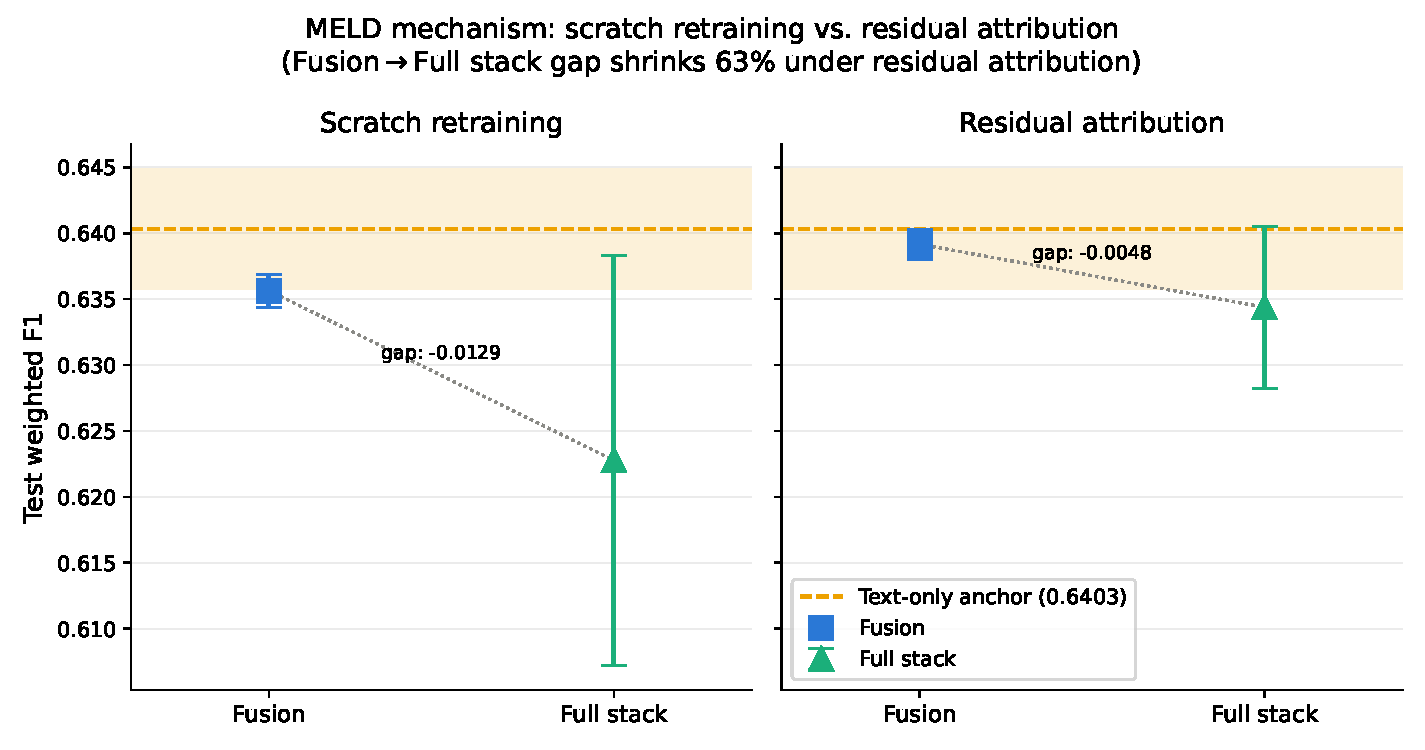
\includegraphics[width=\textwidth]{figures/mechanism_figure.pdf}
\caption{MELD mechanism, two panels at matched scale: test weighted F1 for Fusion and Full stack under scratch retraining (left) versus residual attribution (right), with the Text-only anchor shown as a dashed reference line and a shaded one-standard-deviation band. The Fusion-to-Full-stack gap shrinks $63\%$ under residual attribution (from $-0.0129$ to $-0.0048$), showing that most of the deficit scratch retraining reports is an optimization-and-capacity artifact of that design rather than a property of the components themselves.}
\label{fig:mechanism}
\end{figure*}

The section's conclusion, stated plainly: on MELD, the value of conversation-graph machinery is conditional on a representational deficiency of the foundation beneath it. Reproduce the deficiency and the gains reproduce; repair it (by fine-tuning alone, before any contextual input) and the gains vanish under the most careful attribution we can construct. Section~\ref{sec:iemocap} asks whether a corpus built of long, emotionally volatile dyadic interactions (the pre-registered best case for relationship modeling) changes the verdict.
